Podemos establecer una relación entre las coordenadas rectangulares y las polares mediante la construcción de un punto $(x,y)$ en un plano bidimensional, como se muestra en la siguiente ilustración:

\begin{figure}[H]
  \centering
  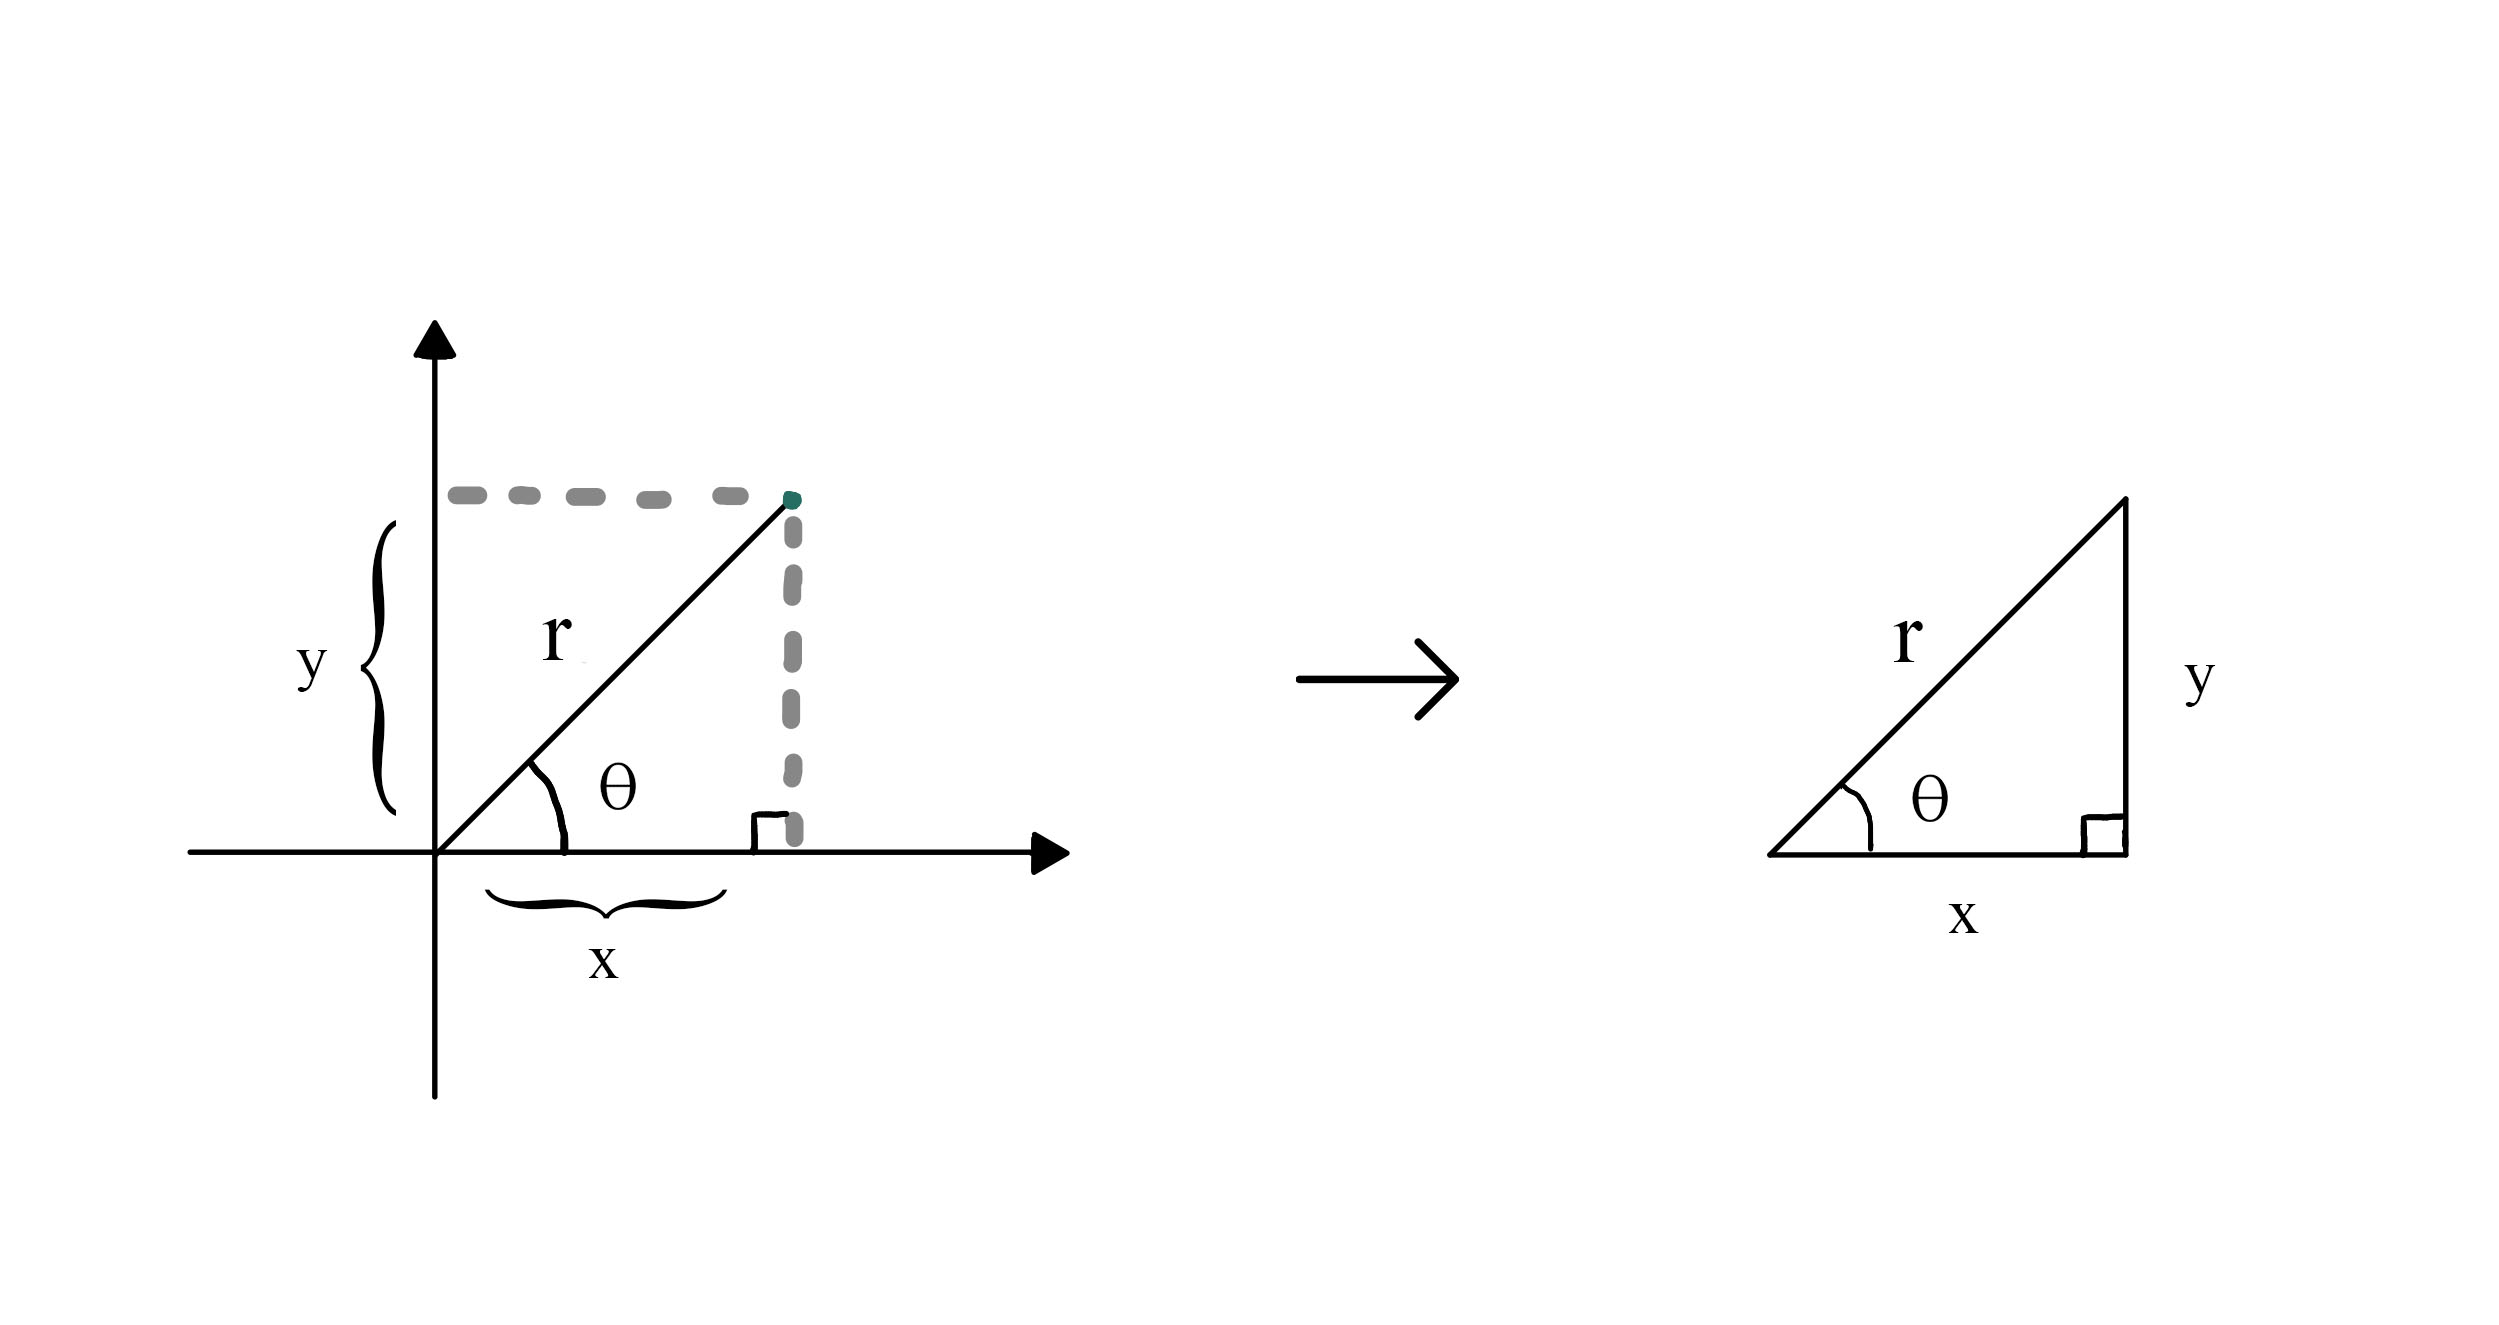
\includegraphics[width=11.17cm, height=5.67cm]{img/graph/relacion_r}
  \caption{Relación de coordenadas rectangulares y polares.}
  \label{relacion_de_coordenadas}
\end{figure}

Donde $r$ representa la distancia desde el origen hasta el punto y el ángulo es $\theta$. Por tanto, existe la coordenada polar $(r,\theta)$, donde el origen permanece igual y el eje polar se representa como el mismo eje x. De ésta manera, se forma un triángulo rectángulo y tenemos las siguientes relaciones:

\[cos\theta = \frac{\text{cateto adyacente}}{\text{hipotenusa}} = \frac{x}{r} \rightarrow x = rcos\theta\]
\[sin\theta = \frac{\text{cateto opuesto}}{\text{hipotenusa}} = \frac{y}{r} \rightarrow y = rsin\theta\]

\vspace{4mm}
Dichas relaciones serán útiles cuando intentemos establecer los métodos de transformación de coordenadas.
